\chapter{Image stitching}
图像拼接应用
\begin{enumerate}
    \item Panorama(全景图)
    \item 360 VR
\end{enumerate}
\section{Image Warping}
一种图像变换. 
\begin{itemize}
    \item Image filtering: 改变强度
    \item Image warping: 改变形状
\end{itemize}
 \subsection{Parametric (global) warping}
 一种全局坐标变换. 
 \begin{align*}
    p'=T(p)
 \end{align*}
 \begin{enumerate}
    \item Linear Transforms = Matrices (线性变换)
    \item Affine Transformatio (仿射变换)
    \begin{enumerate}
        \item Affine map = linear map + translation
        \begin{align*}
            \begin{bmatrix}
                x'\\y'
            \end{bmatrix}=\begin{bmatrix}
                a&b\\c&d
            \end{bmatrix}\begin{bmatrix}
                x\\y
            \end{bmatrix}+\begin{bmatrix}
                t_x\\t_y
            \end{bmatrix}
        \end{align*}
        \item Using homogenous coordinates
        \begin{align*}
            \begin{bmatrix}
                x'\\y'\\1
            \end{bmatrix}=\begin{bmatrix}
                a&b&t_x\\c&d&t_y\\0&0&1
            \end{bmatrix}\begin{bmatrix}
                x\\y\\1
            \end{bmatrix}
        \end{align*}

    \end{enumerate}
    \item Projective Transformation (投影变换)(Homography)(单应)
    \begin{align*}
        \begin{bmatrix}
            x'\\y'\\1
        \end{bmatrix}\cong \begin{bmatrix}
            h_{00}&h_{01}&h_{02}\\
            h_{10}&h_{11}&h_{12}\\
            h_{20}&h_{21}&h_{22}
        \end{bmatrix}\begin{bmatrix}
            x\\y\\1
        \end{bmatrix}
    \end{align*}

    $\begin{bmatrix}
        h_{00}&h_{01}&h_{02}\\
        h_{10}&h_{11}&h_{12}\\
        h_{20}&h_{21}&h_{22}
    \end{bmatrix}$通常范数为1, 所以其一共有8个自由度, 这种问题称之为 up to scale.
    
    其描述为相机平面的改变. Change projection plane (pp).
    \begin{figure}[H]
        \centering
        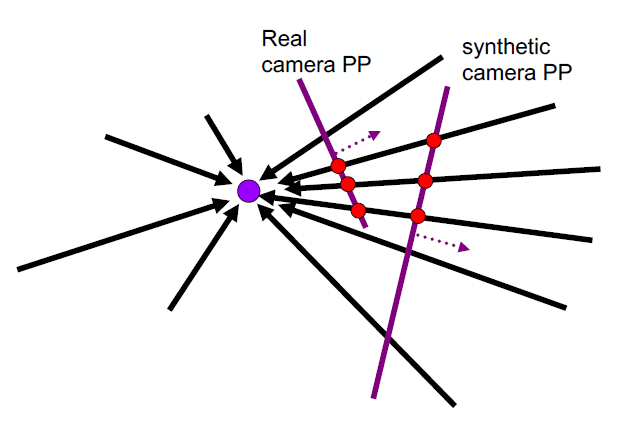
\includegraphics[width=0.33\textwidth]{Lec6/pp}
        \caption{Change projection plane (pp)}
    \end{figure}

    Homography 仅有的情况
    \begin{enumerate}
        \item 相机中心不动, 相机转. (所以拍全景图只能转)
        \item 相机中心移动, 但场景是个平面. 
    \end{enumerate}

    \item Summary of 2D transformations

    \begin{figure}[H]
        \centering
        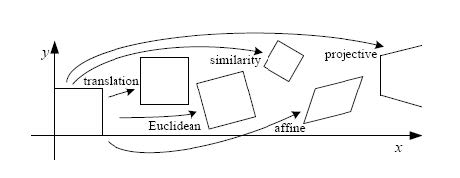
\includegraphics[width=0.33\textwidth]{Lec6/2D transformations}
        \caption{2D transformations}
    \end{figure}
    \item Inverse Transform
    \begin{align*}
        T^{-1}
    \end{align*}
    \begin{figure}[H]
        \centering
        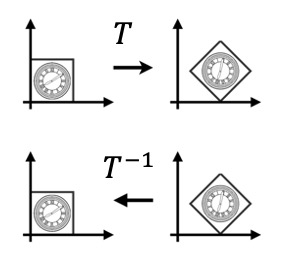
\includegraphics[width=0.33\textwidth]{Lec6/inv}
        \caption{Inverse Transform}
    \end{figure}
 \end{enumerate}

\subsection{Implementing image warping}
实现图像翘曲. Give a coordinate transform $(x', y')=T(x,y)$, and a source image $f(x,y)$.
\begin{figure}[H]
    \centering
    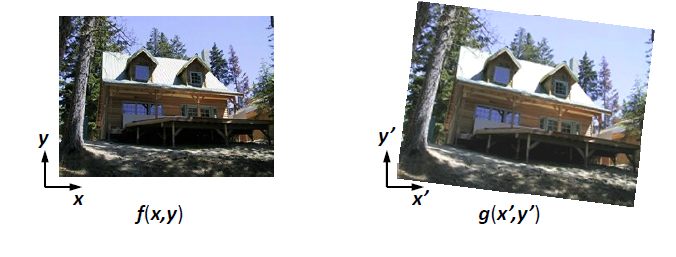
\includegraphics[width=0.33\textwidth]{Lec6/warping}
    \caption{image warping}
\end{figure}

\subsubsection{Forward Warping}
\begin{figure}[H]
    \centering
    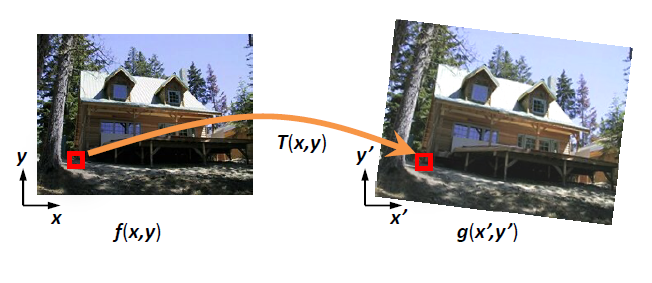
\includegraphics[width=0.33\textwidth]{Lec6/forward}
    \caption{Forward Warping}
\end{figure}

如果算得的值非整数就强行取整, 问题: 有些地方没值. 

\subsubsection{Inverse Warping}
\begin{figure}[H]
    \centering
    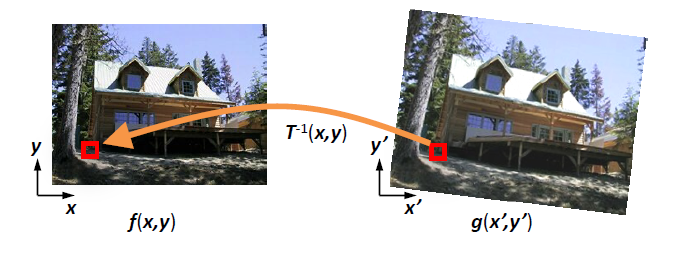
\includegraphics[width=0.33\textwidth]{Lec6/inverse}
    \caption{Inverse Warping}
\end{figure}

反着做保证有值, 如果没值可以插值. (这种高效一点)

\paragraph{Interpolation}
\begin{enumerate}
    \item nearest neighbor
    \item bilinear(一般这个就够了)
    \item bicubic
    \item sinc
\end{enumerate}

\section{Image Stitching}

\subsection{Compute transformation}
\begin{align*}
    \begin{bmatrix}
        x'\\y'\\1
    \end{bmatrix}\cong T \begin{bmatrix}
        x\\y\\1
    \end{bmatrix}
\end{align*}

\begin{figure}[H]
    \centering
    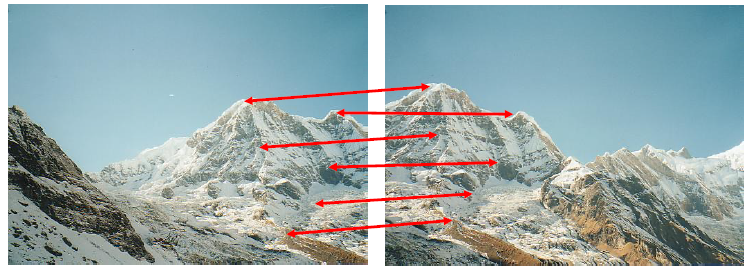
\includegraphics[width=0.33\textwidth]{Lec6/Stitching}
    \caption{Image Stitching}
\end{figure}

\begin{enumerate}
    \item Image matching(每对点有个等式)
    \item 求解 T
\end{enumerate}

\subsubsection{Affine transformations}
每队点两个方程, 共6自由度, 所以要三个方程. 
\begin{align*}
    \begin{bmatrix}
        x'\\y'\\1
    \end{bmatrix}=\begin{bmatrix}
        a&b&c\\d&e&f\\0&0&1
    \end{bmatrix}\begin{bmatrix}
        x\\y\\1
    \end{bmatrix}=\begin{bmatrix}
        ax+by+c\\dx+ey+f\\1
    \end{bmatrix}
\end{align*}

即
\begin{align*}
    x'&=ax+by+c\\
    y'&=dx+ey+f\\
    \begin{bmatrix}
        x'\\y'
    \end{bmatrix}&=\begin{bmatrix}
        x&y&1&0&0&0\\0&0&0&x&y&1
    \end{bmatrix}\begin{bmatrix}
        a\\b\\c\\d\\e\\f
    \end{bmatrix}
\end{align*}

对 n 对点(n matches)
\begin{align*}
    \begin{bmatrix}
        x_1&y_1&1&0&0&0\\0&0&0&x_1&y_1&1\\
        x_2&y_2&1&0&0&0\\0&0&0&x_2&y_2&1\\
        \vdots\\
        x_n&y_n&1&0&0&0\\0&0&0&x_n&y_n&1\\
    \end{bmatrix}\begin{bmatrix}
        a\\b\\c\\d\\e\\f
    \end{bmatrix}&=\begin{bmatrix}
        x'_1\\y'_1\\
        x'_2\\y'_2\\
        \vdots\\
        x'_n\\y'_n\\
    \end{bmatrix}\\
    \underset{2n\times 6}{A} \quad \underset{6\times 1}{t}&=\underset{2n\times 1}{b}
\end{align*}

如果$n\ge3$, 寻找 t,有最小 $\left\| At-b \right\|^2$, 即
\begin{align*}
    A^TAt&=A^Tb\\
    t&=(A^TA)^{-1}A^Tb
\end{align*}

\subsubsection{Projective transformations}

\begin{align*}
    \begin{bmatrix}
        x'_i\\y'_i\\1
    \end{bmatrix}\cong \begin{bmatrix}
        h_{00}&h_{01}&h_{02}\\
        h_{10}&h_{11}&h_{12}\\
        h_{20}&h_{21}&h_{22}
    \end{bmatrix}\begin{bmatrix}
        x_i\\y_i\\1
    \end{bmatrix}
\end{align*}

即
\begin{align*}
    x_{i}^{\prime}&=\frac{h_{00} x_{i}+h_{01} y_{i}+h_{02}}{h_{20} x_{i}+h_{21} y_{i}+h_{22}} \\
    y_{i}^{\prime}&=\frac{h_{10} x_{i}+h_{11} y_{i}+h_{12}}{h_{20} x_{i}+h_{21} y_{i}+h_{22}} \\
\end{align*}
\begin{align*}
    x_{i}^{\prime}\left(h_{20} x_{i}+h_{21} y_{i}+h_{22}\right)&=h_{00} x_{i}+h_{01} y_{i}+h_{02} \\
    y_{i}^{\prime}\left(h_{20} x_{i}+h_{21} y_{i}+h_{22}\right)&=h_{10} x_{i}+h_{11} y_{i}+h_{12}
\end{align*}
\begin{align*}
    \begin{bmatrix}
        x_{i} & y_{i} & 1 & 0 & 0 & 0 & -x_{i}^{\prime} x_{i} & -x_{i}^{\prime} y_{i} & -x_{i}^{\prime} \\
        0 & 0 & 0 & x_{i} & y_{i} & 1 & -y_{i}^{\prime} x_{i} & -y_{i}^{\prime} y_{i} & -y_{i}^{\prime}
    \end{bmatrix}\begin{bmatrix}
        h_{00} \\
        h_{01} \\
        h_{02} \\
        h_{10} \\
        h_{11} \\
        h_{12} \\
        h_{20} \\
        h_{21} \\
        h_{22}
    \end{bmatrix}=\begin{bmatrix}
        0\\0
    \end{bmatrix}
\end{align*}

For n matches,
\begin{align*}
    \begin{array}{cccc}
        \begin{bmatrix}
            x_{1} & y_{1} & 1 & 0 & 0 & 0 & -x_{1}^{\prime} x_{1} & -x_{1}^{\prime} y_{1} & -x_{1}^{\prime} \\
            0 & 0 & 0 & x_{1} & y_{1} & 1 & -y_{1}^{\prime} x_{1} & -y_{1}^{\prime} y_{1} & -y_{1}^{\prime} \\
            \vdots\\
            x_{n} & y_{n} & 1 & 0 & 0 & 0 & -x_{n}^{\prime} x_{n} & -x_{n}^{\prime} y_{n} & -x_{n}^{\prime} \\
            0 & 0 & 0 & x_{n} & y_{n} & 1 & -y_{n}^{\prime} x_{n} & -y_{n}^{\prime} y_{n} & -y_{n}^{\prime}
        \end{bmatrix}&\begin{bmatrix}
            h_{00} \\
            h_{01} \\
            h_{02} \\
            h_{10} \\
            h_{11} \\
            h_{12} \\
            h_{20} \\
            h_{21} \\
            h_{22}
        \end{bmatrix}&=&\begin{bmatrix}
            0\\0\\
            \vdots\\
            0\\0
        \end{bmatrix}\\
        \underset{2n\times 9}{A} & \underset{9\times 1}{t}&=&\underset{2n\times 1}{b}
    \end{array}
\end{align*}

且$\left\| h \right\|=1$

如果$n\ge4$, 寻找 h,有最小 $\left\| Ah-0 \right\|^2$, 即寻找$\hat{h}$, $\hat{h}=(A^TA)$的最小特征值对应的特征向量. 


\subsection{RANSAC}
\begin{enumerate}
    \item Randomly choose s samples
    
    Typically s = minimum sample size that lets you fit a model
    \item Fit a model (e.g., transformation matrix) to those samples
    \item Count the number of inliers that approximately fit the model
    \item Repeat N times
    \item Choose the model that has the largest set of inliers
    \item least squares fit, find average translation vector over all inliers    
    \item 对接缝进行处理, 找接缝附近变化最小的点(Seam insertion)
\end{enumerate}

\subsection{Panorama}
\subsubsection{create}
\begin{enumerate}
    \item Warp all images to a reference image
    \item merge them
\end{enumerate}

但越边缘越小. 

\begin{figure}[H]
    \centering
    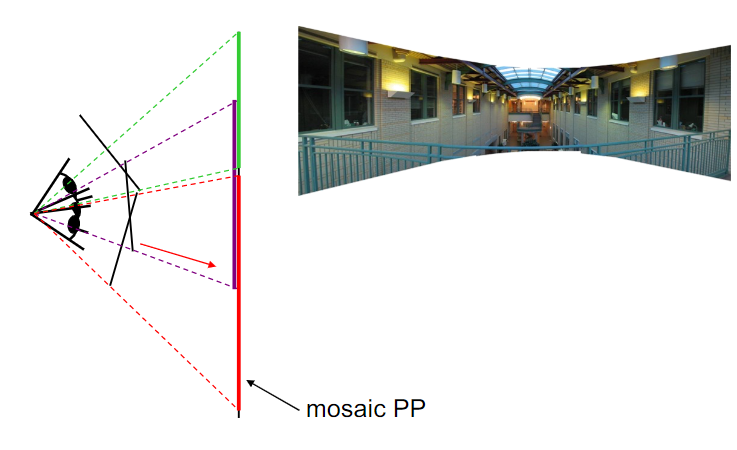
\includegraphics[width=0.28\textwidth]{Lec6/Panorama}
    \caption{Panorama}
\end{figure}

\subsubsection{Cylindrical Panoramas}

可以以相机为中心构造圆柱面, 把其投影到柱面上. 

\begin{figure}[H]
    \centering
    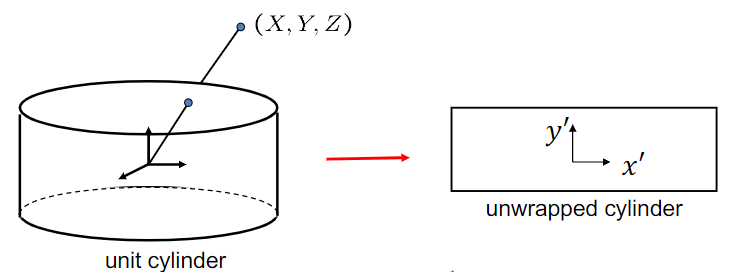
\includegraphics[width=0.28\textwidth]{Lec6/Cylindrical projection}
    \caption{Cylindrical projection}
\end{figure}

\begin{align*}
    x'&=r\tan^-1(\frac{x}{f})\\
    y'&=\frac{ry}{\sqrt{x^2+f^2}}
\end{align*}

$(x', y')$为柱面坐标, $(x, y)$为平面坐标, r为柱半径, f为焦距, 其坐标原点都已移至图像中心.  且相机旋转在柱面上等效于平移. 

\paragraph{Problem: Drift}

误差会累计. 
\begin{figure}[H]
    \centering
    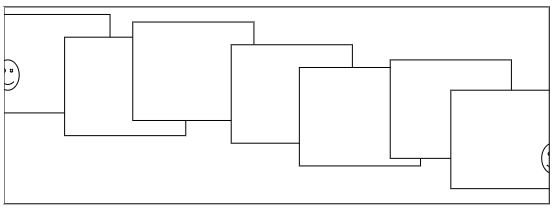
\includegraphics[width=0.28\textwidth]{Lec6/Drift}
    \caption{Drift}
\end{figure}

将首尾特征匹配修正, 转换为优化问题. 
\begin{enumerate}
    \item small (vertical) errors accumulate over time
    \item apply correction so that sum = 0 (for 360° pan.)
\end{enumerate}

因为投影到了柱面, 所以直线会边弯. 